\documentclass[11pt]{article}
\usepackage[margin=1.05in]{geometry}
\usepackage{amsmath,amssymb,amsthm}
\usepackage{booktabs}
\usepackage{array}
\usepackage{tabularx}
\usepackage[protrusion=true,expansion=false]{microtype}
\usepackage[table]{xcolor}
\usepackage{enumitem}
\usepackage{titlesec}
\usepackage{float}
\usepackage{tikz}
\usetikzlibrary{arrows.meta,positioning,calc,backgrounds}
\usepackage{hyperref}

\hypersetup{colorlinks=true, linkcolor=blue!60!black, urlcolor=blue!60!black, citecolor=blue!60!black}
\usepackage[skip=0.6\baselineskip, indent=0pt]{parskip}

\titleformat{\section}{\large\bfseries}{\thesection.}{0.7em}{}
\titleformat{\subsection}{\normalsize\bfseries}{\thesubsection.}{0.6em}{}

\theoremstyle{plain}
\newtheorem{proposition}{Proposition}
\theoremstyle{definition}
\newtheorem{definition}{Definition}

% ----- notation (as in version 0.4, less BLS) -----
\newcommand{\vmax}{V_{\max}}
\newcommand{\Tc}{T_{\mathrm{close}}}
\newcommand{\bcorr}{b_{\mathrm{corr}}}
\newcommand{\tx}[1]{\texttt{#1}}
\newcommand{\be}[2]{\langle #1\rangle_{#2}}
\newcommand{\pre}[2]{[#1]_{#2}}
\newcommand{\xo}[1]{\mathsf{x}(#1)}
\newcommand{\Ht}[1]{H_{\textsf{#1}}}
\newcommand{\Sign}{\mathsf{Sign}}
\newcommand{\Vfy}{\mathsf{Verify}}
\newcommand{\PSign}{\mathsf{PreSign}}
\newcommand{\PVfy}{\mathsf{PreVerify}}
\newcommand{\Compl}{\mathsf{Complete}}
\newcommand{\Extr}{\mathsf{Extract}}
\newcommand{\Wots}{\mathsf{W}}
\newcommand{\kiss}{k_{\mathrm{iss}}}
\newcommand{\Piss}{P_{\mathrm{iss}}}
\newcommand{\owed}{\mathsf{owed}}
\newcommand{\PH}{P_H^{c}}
\newcommand{\Oc}{O_c}
\newcommand{\KQ}{K_{Q}^{c}}
\newcommand{\Kb}{K_{b}^{c}}
\newcommand{\Kcorr}{K_{\mathrm{corr}}^{c}}
\newcommand{\KU}{K_{U}^{c}}
\newcommand{\Acorr}{A_{\mathrm{corr}}^{c}}
\newcommand{\AU}{A_{U}^{c}}
\newcommand{\kin}{k_{\mathrm{in}}}
\newcommand{\vin}{v_{\mathrm{in}}}
\newcommand{\vout}{v_{\mathrm{out}}}

\newcolumntype{L}{>{\raggedright\arraybackslash}X}
\renewcommand{\arraystretch}{1.3}
\makeatletter
\setlength{\@fptop}{0pt}
\setlength{\@fpsep}{1.5\baselineskip}
\setlength{\@fpbot}{0pt plus 1fil}
\makeatother

\newenvironment{algobox}[1]
  {\par\smallskip\noindent\begin{tabular}{|p{0.955\linewidth}|}\hline\textbf{#1}\\[2pt]}
  {\\\hline\end{tabular}\par\smallskip}

\title{\textbf{The grants L2}\\a Lichen L2 without global order\\[2pt]\large early draft: one note per account, in sequence}
\author{waxwing}
\date{Version 0.5, November 2026\\[2pt]\small a companion to \emph{Lichen}, version 0.5~\cite{lichen}, and an alternative to version 0.4~\cite{grants04}}

\begin{document}
\maketitle

\begin{abstract}
Version 0.4 of the grants L2~\cite{grants04} lets a user hold many notes
and protects at most four of them in an exit. Its limits follow from
that: claims of up to four notes and fallbacks, a fixed point over sets
to count them, merges that need the hub, BLS aggregation to keep a claim
small, and a hub that gains by halting while users hold more notes than
a claim can carry.

This version gives each key exactly one note at a time, numbered in
sequence: $(o, k, v)$, owner, sequence number, value. A payment is a
\emph{joint spend} that moves the payer's account and the payee's each
one step on, and both sign it; one grant opens both new notes. The payee
must be online to be paid, like a Lightning payee. Each account is
ordered and the system is not: there is no global order, no sequencer,
no anchoring. The order within an account does the rest. A claim is one
note, 74 bytes on chain. The hub answers any claim by citing one spend:
a later step of the same account supersedes the claimed one, so a
spend in flight needs no naming and a stale claim never pays more than
a current one. Algorithm~1 has two cases; there are no transaction ids,
no merges and no fallbacks; a halting hub has nothing to keep; user and
hub each store only the latest state of an account. With one note per
claim there is nothing to aggregate, so notes are signed with BIP340 and
encrypted by adaptor, and the hub's statement needs no pairing: about
1.7M cycles (estimated), against 29M. The exit's graph is version
0.4's, its three exit transactions 45--70\% smaller. A deferred receipt
through a mailbox is set apart as an option (\S\ref{sec:deferred}). A
proposal; nothing here is built.
\end{abstract}

\tableofcontents

\section{Setting}

The setting is version 0.4's~\cite{grants04}. A Lichen contract
(\cite{lichen}, \S3) locks the hub's liquidity and the user's deposit in
one Bitcoin output, with a cap $\vmax$, reserves $r_A$ and $r_H$, a
close time $\Tc$ and a unit $u$ (sats per unit; an on-chain amount $b$
is a 4-byte word paid out as $u\,b$ sats). It ends by \textbf{fold}
(both sign), \textbf{default} (after $\Tc$: she gets $r_A$) or
\textbf{exit} (she claims $b$; she is paid $b$, or the hub's correction
$\bcorr \le b$ if the hub proves her owed no more). The hub's book is the
only ledger.

\textbf{Contracts and credit.} A user's participation is defined by her
contract. Contract $c$ has a fresh L2 key $\Oc$; the note of $\Oc$ is
what $c$'s exit claims. A note under any other key is credit.

\textbf{Accounts.} Each key is an \emph{account}: a sequence of notes,
numbered $0, 1, 2, \dots$, of which exactly one is live. Receiving is a
step of the receiver's account, so the receiver signs it. Accounts are
ordered one by one and not against each other: a payment advances two
accounts at once, and nothing relates Alice's numbers to Bob's.

\section{Notation}\label{sec:notation}

As in version 0.4 (\cite{grants04}, \S2), with BLS12-381 removed.

\begin{itemize}[nosep]
\item secp256k1: generator $G$, order $n$; every key x-only
  (BIP340~\cite{bip340}). Lower-case letters scalars, upper-case points.
  $\xo{P}$ the 32-byte x-coordinate; $P^{(33)}$ the point compressed.
\item $\be{v}{k}$: $v$ as $k$ bytes, big-endian. $\pre{h}{k}$: the first
  $k$ bytes of $h$. $\|$: concatenation.
\item $\Ht{tag}(p_1, \dots, p_r)$: the L2's tagged hash, SHA-256 over the
  tag \textsf{lichen/notes/\ldots}, a zero byte, and each part
  length-prefixed. Tags \textsf{note}, \textsf{half}, \textsf{spend},
  \textsf{auth}, \textsf{unlock}, \textsf{unlock-scalar}.
\item BIP340: $\Sign_d(m)$, $\Vfy_P(m, \sigma)$, 64 bytes. An owner's
  signature on a spend is written $\psi$, the issuer's on a note
  $\sigma$.
\end{itemize}

\textbf{Adaptor signatures}~\cite{poelstra,aumayr} replace version 0.4's
BLS encryption. For a point $T = tG$, the issuer's pre-signature on $m$
is $\rho = \PSign_{\kiss}(m, T) = (R', s')$: it draws $k$ until $R = kG
+ T$ has even $y$, sets $R' = kG$ and $s' = k + e(R, \Piss, m)\,\kiss$.
$\PVfy_{\Piss}(m, T, \rho)$ holds iff $s'G = R' + e(R' + T, \Piss,
m)\Piss$ and $R' + T$ has even $y$. $\Compl(\rho, t) = (\xo{R' + T},\ s'
+ t)$ is an ordinary BIP340 signature on $m$, and $\Extr(\sigma, \rho) =
s - s'$ gives $t$ back. A pre-signature is 65 bytes ($R'$ compressed,
$s'$).

Version 0.4 chose BLS because four notes aggregate to one 48-byte
signature, and, BLS being unique and so without adaptors
(\cite{grants04}, \S2.2), it encrypted signatures instead. With one note
per claim nothing aggregates, and with BIP340 notes adaptors are
standard: the statement verifies BIP340, which RISC Zero accelerates,
instead of a pairing. That $\Extr$ recovers $t$ costs nothing: $t$
always travels in the clear (\S\ref{sec:payment}).

\textbf{One-time signatures} $\Wots_K(x)$: as in version 0.4. Winternitz,
4-bit digits plus checksum, 2 witness items a digit; SHA-256 chains for
Alice's keys, HASH160 for the hub's; two different signatures under one
key are an \emph{equivocation}.

\textbf{Keys.}
\begin{center}
\begin{tabularx}{\linewidth}{llL}
\toprule
Symbol & Scope & Use \\
\midrule
$\kiss$, $\Piss = \kiss G$ & the deployment & the issuer's key: signs every note; pre-signs every grant's new notes \\
$\PH$, $P_A^c$ & contract $c$ & the 2-of-2 on every link of $c$'s graph \\
$a_c$, $\Oc = a_cG$ & contract $c$ & her L2 key, fresh for $c$: owns $c$'s account; signs its steps \\
$\KQ$, $\Kb$, $\Acorr$, $\AU$ & contract $c$, hers & one-time: $Q$ and $b$ in \tx{request}; her countersignatures in \tx{ack} \\
$\Kcorr$, $\KU$ & contract $c$, the hub's & one-time: $\bcorr$ and $U$ in \tx{correct} \\
$z_S$, $t_S$, $T_S = t_S G$ & spend $S$ & the unlock: a 16-byte seed, its scalar, its point \\
\bottomrule
\end{tabularx}
\end{center}

\section{Accounts, spends and grants}

\subsection{Notes}\label{sec:notes}

\begin{definition}
A \emph{note} is $N = (o, k, v)$: an owner, a sequence number $0 \le k <
2^{32}$, and a value $0 \le v < 2^{48}$ sats. Its digest is $\delta(N) =
\Ht{note}(o, \be{k}{4}, \be{v}{8})$. It is \emph{settled} when its
holder has $\sigma_N = \Sign_{\kiss}(\delta(N))$.
\end{definition}

\textbf{Every account starts at 0.} A contract key's note 0 is its
\emph{mint}, $(\Oc, 0, v_0)$, which the contract vouches for
(\S\ref{sec:contract}); any other key's note 0 is the empty note $(o, 0,
0)$. Neither needs a signature. Each spend an account takes part in
moves it from $k$ to $k + 1$. A value may be 0: a payer who spends her
whole balance keeps a note of 0, and her account goes on.

\textbf{No ids.} A note is named by its owner and number, which are
unique as long as each account has one live note. So the
32-byte ids of version 0.4, its 16-byte short ids, and the output ids
derived from a spend's id are all gone, and with them the argument that
a payer can't grind two payments to one payee into the same short id:
numbers are assigned, not chosen.

\textbf{The invariant: one live note per account.} The hub keeps it by
recording a spend only if it takes each owner's live note; the owner
keeps it by signing only spends of the note she holds (Rule 3,
\S\ref{sec:rules}).

\subsection{Spends, in halves}\label{sec:spend}

\begin{definition}
A \emph{half} for owner $o$ is $\eta = (o,\ \kin,\ \vin,\ \vout,\
\lambda)$: $o$'s note $(o, \kin, \vin)$, the value $\vout$ it leaves
with, and a 16-byte blinding $\lambda$ that $o$ chooses. Its digest is
\[
  h(\eta) = \Ht{half}\big(o,\ \be{\kin}{4},\ \be{\vin}{8},\
  \be{\vout}{8},\ \lambda\big),
\]
and its \emph{step} gives $o$ the note $(o, \kin + 1, \vout)$.

A \emph{spend} $S$ is two halves with distinct owners, $o_1 < o_2$ as
bytes. It is well formed if $v_{\mathrm{in},1} + v_{\mathrm{in},2} =
v_{\mathrm{out},1} + v_{\mathrm{out},2}$ and each half's note is its
owner's live one. Its digest, the message both owners approve, is
\[
  \delta(S) = \Ht{spend}\big(o_1,\ h(\eta_1),\ o_2,\ h(\eta_2)\big).
\]
\end{definition}

$\delta(S)$ is a hash of the spend's contents, as any signed message is
hashed. It is not an identifier: no note records it, no claim posts it,
and nothing refers to it. A spend is named, if it needs naming, by the
two notes it takes, $(o_1, k_1)$ and $(o_2, k_2)$: each note is taken
once, so the pair is unique.

A payment of $a$ from Alice, holding $(o_A, k_A, v_A)$, to Bob, holding
$(o_B, k_B, v_B)$, has the halves $(o_A, k_A, v_A, v_A - a, \lambda_A)$
and $(o_B, k_B, v_B, v_B + a, \lambda_B)$.

\textbf{Halves hide balances from the counterparty.} Each party sees
its own half and the other's digest. Both know $a$; neither learns the
other's balance or number. The blinding keeps the digest from being
searched by anyone who knows the owner and could guess the values. The
hub sees both halves and checks that the values balance; the statement
never needs to (\S\ref{sec:statement}).

\subsection{Grants}\label{sec:grant}

\begin{definition}
The hub's \emph{grant} on a well-formed spend $S$ is $\Gamma = (T_S,\
\rho_1,\ \rho_2)$, with
\begin{gather*}
  z_S = \pre{\Ht{unlock}(\kiss, \delta(S))}{16},\qquad T_S = t_S G,\\
  t_S = \Ht{unlock-scalar}(z_S, \be{\mathit{ctr}}{4})\ \ (\text{the least
  } \mathit{ctr} \text{ with } 0 < t_S < n),\\
  \rho_i = \PSign_{\kiss}\big(\delta(o_i, k_{\mathrm{in},i} + 1,
  v_{\mathrm{out},i}),\ T_S\big),\qquad i = 1, 2,
\end{gather*}
the pre-signatures on the two new notes. The message both owners sign is
\[
  \alpha = \Ht{auth}\big(\delta(S),\ T_S^{(33)},\ \rho_1^{(65)},\
  \rho_2^{(65)}\big).
\]
\end{definition}

Each owner checks the pre-signature on its own new note and signs
$\alpha$ over the other's as bytes. Both sign one $\alpha$, so they
agree on $T_S$: version 0.4's $\tau$ and its commitment $C$, which
served a payee who saw only part of the grant, have no role left.

\begin{definition}
An exit's \emph{unlock} $U$ is one 16-byte seed: that of the spend the
hub cites against the claim, or zeros if it cites none
(\S\ref{sec:volume}).
\end{definition}

\section{A payment}\label{sec:payment}

\subsection{Live receipt}\label{sec:live}

Figure~\ref{fig:payment}. Bob gives Alice an invoice $(o_B, a)$; both
are online.

\begin{figure}[!tbp]
\centering
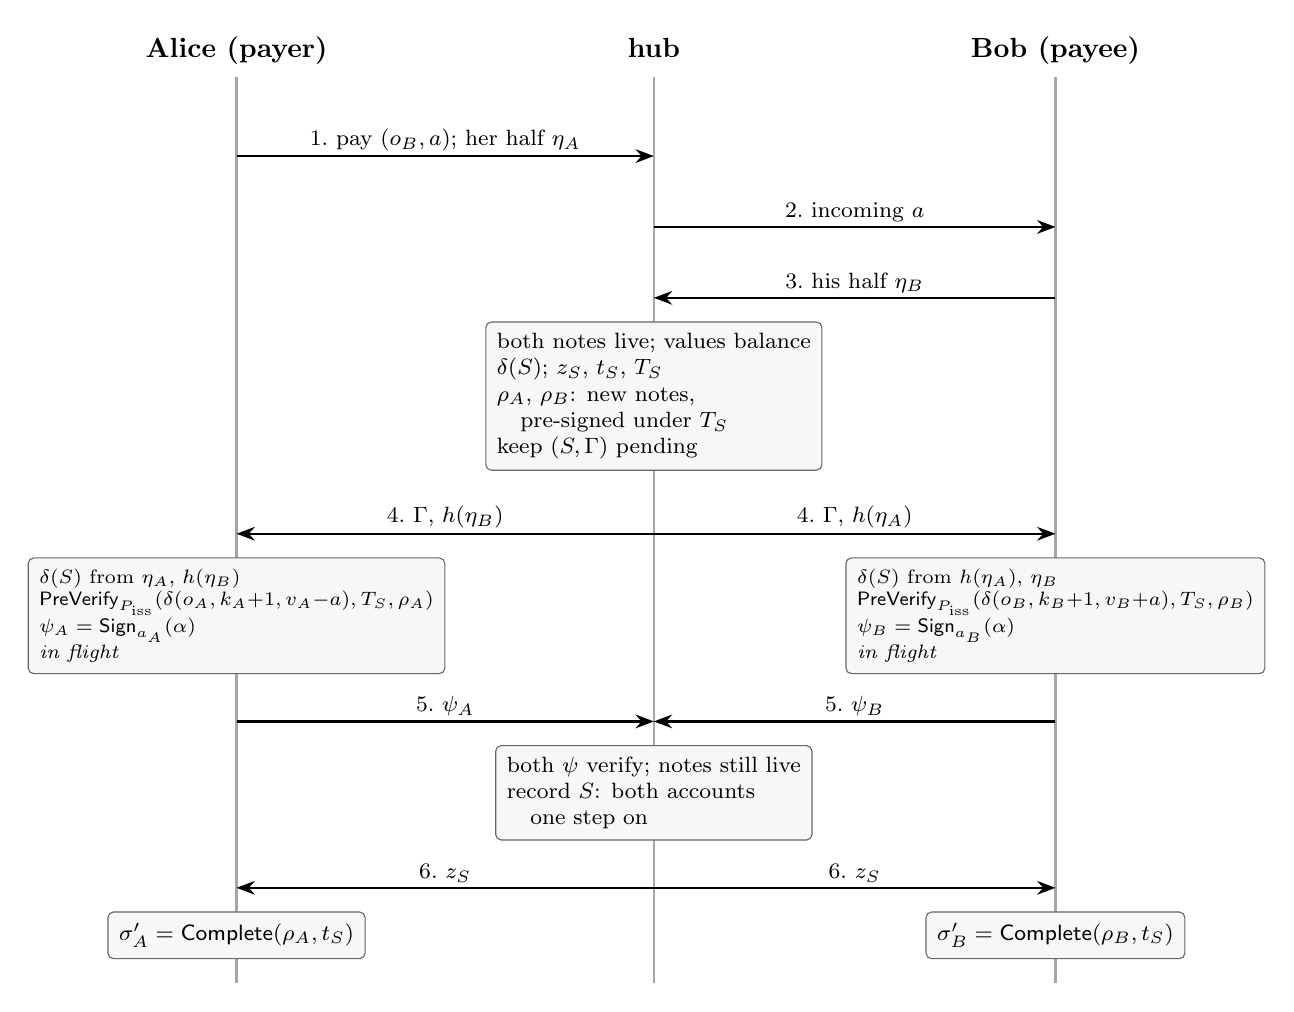
\begin{tikzpicture}[>=Stealth, font=\small,
  life/.style={draw=black!35, thick},
  box/.style={draw=black!60, fill=black!3, rounded corners=2pt, align=left, inner sep=4pt, font=\footnotesize},
  msg/.style={->, thick},
  lbl/.style={align=center, font=\footnotesize, inner sep=1.5pt}]
\coordinate (LA) at (2.7,0); \coordinate (LH) at (8.0,0); \coordinate (LB) at (13.1,0);
\node[font=\bfseries, anchor=base] at ($(LA)+(0,0.25)$) {Alice (payer)};
\node[font=\bfseries, anchor=base] at ($(LH)+(0,0.25)$) {hub};
\node[font=\bfseries, anchor=base] at ($(LB)+(0,0.25)$) {Bob (payee)};
\coordinate (y) at (0,-1.0);
\draw[msg] (LA|-y) -- node[lbl, above] {1.\ pay $(o_B, a)$; her half $\eta_A$} (LH|-y);
\coordinate (y) at ($(y)+(0,-0.9)$);
\draw[msg] (LH|-y) -- node[lbl, above] {2.\ incoming $a$} (LB|-y);
\coordinate (y) at ($(y)+(0,-0.9)$);
\draw[msg] (LB|-y) -- node[lbl, above] {3.\ his half $\eta_B$} (LH|-y);
\node[box, anchor=north] (b1) at ($(LH|-y)+(0,-0.3)$) {
  both notes live; values balance\\
  $\delta(S)$; $z_S$, $t_S$, $T_S$\\
  $\rho_A$, $\rho_B$: new notes,\\ \quad pre-signed under $T_S$\\
  keep $(S, \Gamma)$ pending};
\coordinate (y) at ($(b1.south)+(0,-0.8)$);
\draw[msg] (LH|-y) -- node[lbl, above] {4.\ $\Gamma$, $h(\eta_B)$} (LA|-y);
\draw[msg] (LH|-y) -- node[lbl, above] {4.\ $\Gamma$, $h(\eta_A)$} (LB|-y);
\node[box, anchor=north, font=\scriptsize] (b2) at ($(LA|-y)+(0,-0.3)$) {
  $\delta(S)$ from $\eta_A$, $h(\eta_B)$\\
  $\PVfy_{\Piss}(\delta(o_A, k_A{+}1, v_A{-}a), T_S, \rho_A)$\\
  $\psi_A = \Sign_{a_A}(\alpha)$\\
  \emph{in flight}};
\node[box, anchor=north, font=\scriptsize] (b3) at ($(LB|-y)+(0,-0.3)$) {
  $\delta(S)$ from $h(\eta_A)$, $\eta_B$\\
  $\PVfy_{\Piss}(\delta(o_B, k_B{+}1, v_B{+}a), T_S, \rho_B)$\\
  $\psi_B = \Sign_{a_B}(\alpha)$\\
  \emph{in flight}};
\coordinate (y) at ($(b2.south)+(0,-0.6)$);
\draw[msg] (LA|-y) -- node[lbl, above] {5.\ $\psi_A$} (LH|-y);
\draw[msg] (LB|-y) -- node[lbl, above] {5.\ $\psi_B$} (LH|-y);
\node[box, anchor=north] (b4) at ($(LH|-y)+(0,-0.3)$) {
  both $\psi$ verify; notes still live\\
  record $S$: both accounts\\ \quad one step on};
\coordinate (y) at ($(b4.south)+(0,-0.6)$);
\draw[msg] (LH|-y) -- node[lbl, above] {6.\ $z_S$} (LA|-y);
\draw[msg] (LH|-y) -- node[lbl, above] {6.\ $z_S$} (LB|-y);
\node[box, anchor=north] (b5) at ($(LA|-y)+(0,-0.3)$) {$\sigma'_A = \Compl(\rho_A, t_S)$};
\node[box, anchor=north] (b6) at ($(LB|-y)+(0,-0.3)$) {$\sigma'_B = \Compl(\rho_B, t_S)$};
\coordinate (end) at ($(b5.south)+(0,-0.3)$);
\begin{scope}[on background layer]
\foreach \l in {LA,LH,LB} \draw[life] (\l) -- (\l|-end);
\end{scope}
\end{tikzpicture}
\caption{A live payment: one step of each account. Each party is in
flight from its signature (step 5) until it has $z_S$ (step 6). Either
can hand $z_S$ to the other.}
\label{fig:payment}
\end{figure}

The payment is complete for a party when it holds $z_S$: its new note
is then settled. Alice's receipt is $z_S$; Bob's acceptance is his
$\psi_B$, which the hub can show her. Either party holding $z_S$ can
hand it to the other, so neither depends on the hub to learn that the
other side completed.

\textbf{In flight.} From its signature until it holds $z_S$, a party
keeps its old note and $(S, \Gamma)$. It needs nothing else. Its claim
names the old note, and if the hub uses $S$ against that claim, it must
publish $z_S$, and the new note counts (\S\ref{sec:claim}).

\subsection{Rules}\label{sec:rules}

\textbf{Rule 1 (the statement): a spend counts only with both owners'
signatures.} A cited spend is usable only if $\psi_1$ and $\psi_2$ both
verify on $\alpha$ (\S\ref{sec:statement}). Without it, the hub could
take $\psi_A$ alone, cite $S$ against Alice, and publish $z_S$ to a Bob
who never signed, and so may not hold the grant: she would be debited
and no one paid. With it, $S$ counts against no one until both have
signed; and both signers hold the grant, so whichever exit publishes
$z_S$ settles both new notes.

\textbf{Rule 2 (the wallet): one pending signature per account.} A
wallet never signs a spend while another it signed is pending. If Bob
signed two incoming payments that both take his note $k$, the hub could
complete both and count each against its payer, while Bob's account
moves to $k+1$ only once. The hub can't make a wallet break this rule.
It means one payment at a time per account, in either direction; an
honest hub tells a second payer \emph{busy, retry}.

\textbf{Rule 3 (the wallet): sign only steps from the note you hold.}
Each owner checks its half: $(o, \kin, \vin)$ is its live note, and
$\vout$ the value it expects. So the account's invariant is the owner's
own, whatever the hub does, and every spend she ever signs has $\kin$ at
most her current number.

\textbf{Cancelling.} A party in flight asks the hub to cancel. If the
hub holds both signatures, it answers with $z_S$: the payment is done.
Otherwise it \emph{reissues} the party's note one step on, $(o, k + 1,
v)$, the same value with $\sigma$; and refuses $S$ from then on. The
party holds the reissue and nothing in flight. If the hub completed $S$
anyway, $S$ takes note $k$, which is behind the reissue: it can't count
against a claim of the reissue (\S\ref{sec:algo}), and the hub has paid
the counterparty from nothing. So a reissue needs no certificate: it is
just the account's next note.

\subsection{What atomicity means here}\label{sec:atomic}

Once both have signed, the hub may record $S$ or not.
\begin{itemize}[nosep]
\item Not recorded, or cancelled: the hub alone knows $t_S$; the new
  notes never settle, and the old ones (or their reissues) stand.
\item Recorded, $z_S$ given to either party: both are paid, since the
  other can be handed $z_S$.
\item Recorded, $z_S$ withheld from both: both are in flight, and
  neither exit can be reduced through $S$ without publishing $z_S$,
  which settles both new notes.
\end{itemize}
Version 0.4's atomicity was one-way: the chain enforced the payer's
side, and the payee was paid once he held a settled note. Here both
parties step their accounts by one spend, and are protected the same
way.

\textbf{Settling into a closed contract.} One gap remains, and version
0.4 has it too. Suppose the hub records $S$, withholds $z_S$, and Bob
exits first. The hub doesn't cite $S$ against him (it would raise what
he is owed), so he is paid his old note. Later the hub cites $S$ against
Alice: she is debited $a$, and Bob's new note settles under a key whose
contract has closed, as credit. The hub keeps $a$. Order is what
matters: had Alice exited first, $S$ would either have been cited,
settling Bob's note while his contract was open, or not, leaving both
whole. So the rule for a halt is \textbf{payers exit first}: a payee
with an incoming payment in flight waits for its payer's exit to pass
\tx{correct} (or its window), as long as its own close allows. Both are
online parties to the payment, so they can arrange it. At stake: at
most one payment per account, and only one the hub has deliberately
left pending.

\section{The contract}\label{sec:contract}

\textbf{Opening and the mint} are version 0.4's (\cite{grants04},
\S4.1), with the mint renamed: note 0 of $\Oc$, $(\Oc, 0, v_0)$, exists
exactly when the funding transaction confirms, and its evidence is the
journal, which binds $v_0$. The hub refuses an $\Oc$ it has seen before,
so the account is new.

\textbf{The journal}, the statement's public input:
\begin{align*}
  J &= \be{c}{4} \,\|\, D,\qquad
  D = \mathrm{SHA256}\big(\texttt{"lichen/grants/contract"} \,\|\,
  \xo{\Piss} \,\|\, \xo{\Oc} \,\|\, \be{u}{8} \,\|\, \be{v_0}{8} \,\|\,
  \kappa\big),\\
  \kappa &= \mathrm{SHA256}\big(\KQ \,\|\, \Kb \,\|\, \Acorr \,\|\, \AU\big).
\end{align*}
Only the issuer's key changes from version 0.4: a secp256k1 key in
place of BLS's $I$.

\textbf{The dispute graph} is version 0.4's unchanged
(Figure~\ref{fig:graph}; \cite{grants04}, \S4.3--4.4): payouts in bits,
each bit output spent by re-presenting the one-time signature on the
amount, with an equivocation leaf for the other party. Only the lengths
change: $Q$ is 74 bytes and $U$ 16 (\S\ref{sec:costs}).

\begin{figure}[!tbp]
\centering
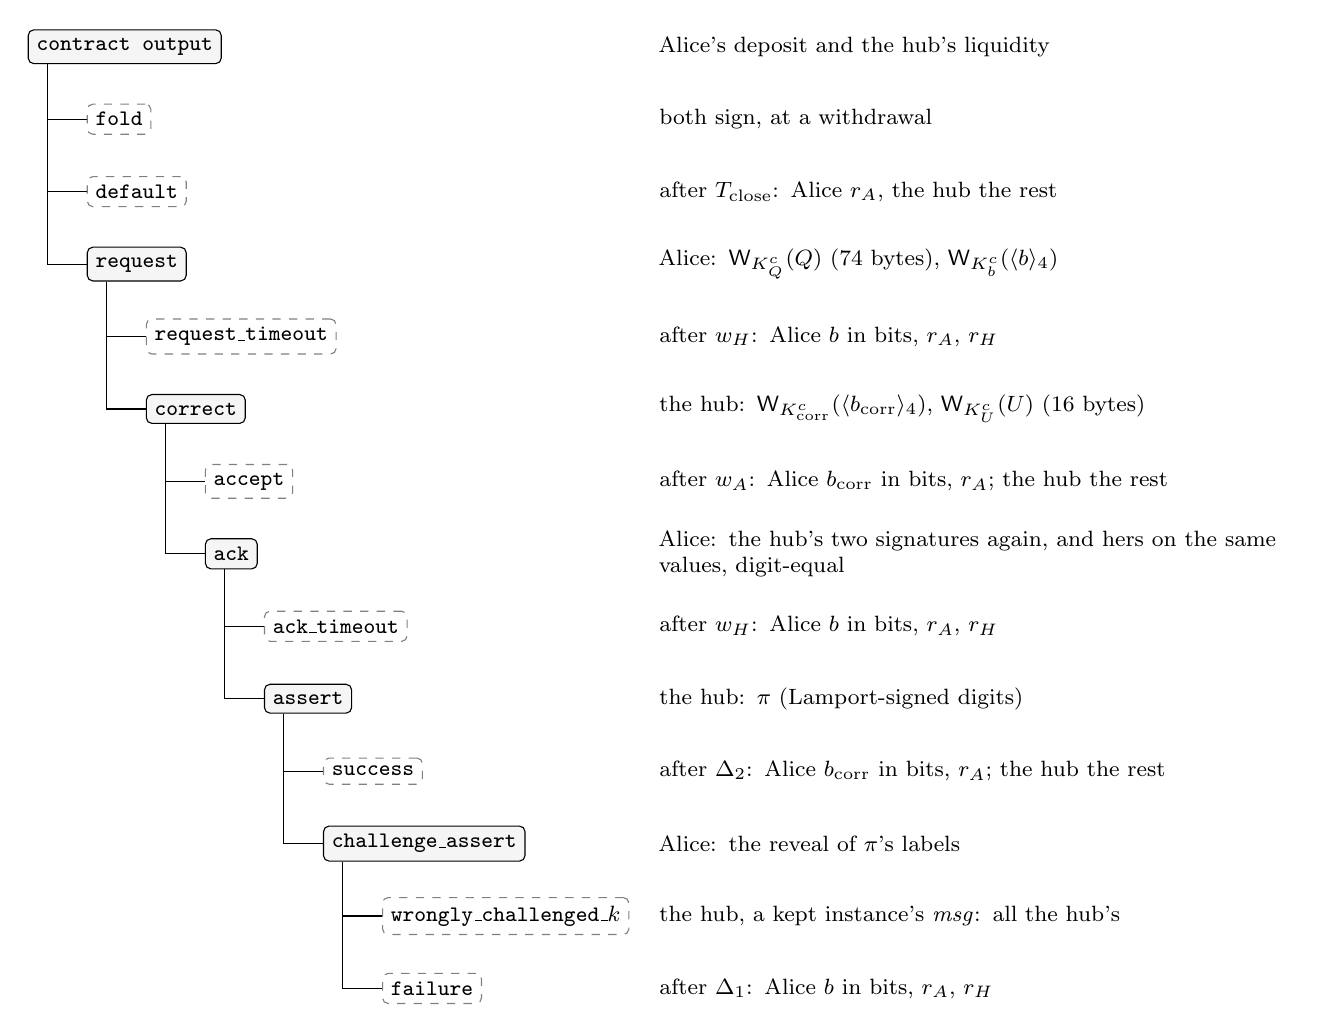
\begin{tikzpicture}[font=\footnotesize,
  link/.style={draw, rounded corners=2pt, inner sep=3pt, fill=black!4, font=\footnotesize\ttfamily, anchor=west},
  term/.style={draw=black!50, dashed, rounded corners=2pt, inner sep=3pt, font=\footnotesize\ttfamily, anchor=west},
  ann/.style={anchor=west, align=left, text width=7.9cm, font=\footnotesize}]
\def\dx{0.75}\def\dy{0.92}\def\ax{7.9}
\node[link] (c)  at (0*\dx, 0)       {contract output};
\node[term] (fo) at (1*\dx, -1*\dy)  {fold};
\node[term] (de) at (1*\dx, -2*\dy)  {default};
\node[link] (rq) at (1*\dx, -3*\dy)  {request};
\node[term] (rt) at (2*\dx, -4*\dy)  {request\_timeout};
\node[link] (co) at (2*\dx, -5*\dy)  {correct};
\node[term] (ac) at (3*\dx, -6*\dy)  {accept};
\node[link] (ak) at (3*\dx, -7*\dy)  {ack};
\node[term] (at) at (4*\dx, -8*\dy)  {ack\_timeout};
\node[link] (as) at (4*\dx, -9*\dy)  {assert};
\node[term] (su) at (5*\dx, -10*\dy) {success};
\node[link] (ch) at (5*\dx, -11*\dy) {challenge\_assert};
\node[term] (wc) at (6*\dx, -12*\dy) {wrongly\_challenged\_$k$};
\node[term] (fa) at (6*\dx, -13*\dy) {failure};
\foreach \p/\q in {c/fo,c/de,c/rq,rq/rt,rq/co,co/ac,co/ak,ak/at,ak/as,as/su,as/ch,ch/wc,ch/fa}
  \draw ($(\p.south west)+(0.25,0)$) |- (\q.west);
\node[ann] at (\ax, 0)         {Alice's deposit and the hub's liquidity};
\node[ann] at (\ax, -1*\dy)    {both sign, at a withdrawal};
\node[ann] at (\ax, -2*\dy)    {after $\Tc$: Alice $r_A$, the hub the rest};
\node[ann] at (\ax, -3*\dy)    {Alice: $\Wots_{\KQ}(Q)$ (74 bytes), $\Wots_{\Kb}(\be{b}{4})$};
\node[ann] at (\ax, -4*\dy)    {after $w_H$: Alice $b$ in bits, $r_A$, $r_H$};
\node[ann] at (\ax, -5*\dy)    {the hub: $\Wots_{\Kcorr}(\be{\bcorr}{4})$, $\Wots_{\KU}(U)$ (16 bytes)};
\node[ann] at (\ax, -6*\dy)    {after $w_A$: Alice $\bcorr$ in bits, $r_A$; the hub the rest};
\node[ann] at (\ax, -7*\dy)    {Alice: the hub's two signatures again, and hers on the same values, digit-equal};
\node[ann] at (\ax, -8*\dy)    {after $w_H$: Alice $b$ in bits, $r_A$, $r_H$};
\node[ann] at (\ax, -9*\dy)    {the hub: $\pi$ (Lamport-signed digits)};
\node[ann] at (\ax, -10*\dy)   {after $\Delta_2$: Alice $\bcorr$ in bits, $r_A$; the hub the rest};
\node[ann] at (\ax, -11*\dy)   {Alice: the reveal of $\pi$'s labels};
\node[ann] at (\ax, -12*\dy)   {the hub, a kept instance's \textit{msg}: all the hub's};
\node[ann] at (\ax, -13*\dy)   {after $\Delta_1$: Alice $b$ in bits, $r_A$, $r_H$};
\end{tikzpicture}
\caption{A contract's graph, as in version 0.4: solid boxes carry the
value on, dashed ones are terminals.}
\label{fig:graph}
\end{figure}

\textbf{Withdrawal.} Alice hands the hub her claim (\S\ref{sec:claim})
signed with $a_c$. The hub takes it if the note is her account's live
one: it marks the account closed, and both sign the fold, which pays her
$u\,b$ and $r_A$. What the note held beyond $u\,b$ the hub issues to
her wallet's key with no contract, as credit.

\section{The exit}\label{sec:exit}

\subsection{The claim}\label{sec:claim}

\begin{definition}
A \emph{claim} on contract $c$ is $(b;\ k, v, \sigma)$: a note of her
account, $(\Oc, k, v)$, with its signature (none for $k = 0$, the mint,
whose value is $v_0$); and $b \le \lfloor v/u \rfloor$.
\end{definition}

An honest wallet claims its live note. If it has a spend in flight, it
still claims the note that spend takes: the step, if the hub uses it,
counts by itself (\S\ref{sec:algo}).

\textbf{The posted claim} $Q$, exactly $L_Q = 74$ bytes:
\[
  Q = \be{k}{4} \,\|\, \be{v}{6} \,\|\, \sigma^{(64)},
\]
zeros in place of $v$ and $\sigma$ when $k = 0$. The owner, the contract
and $v_0$ come from the journal; $b$ is signed under its own key, as in
version 0.4.

A claim covers the whole balance of the account. There is no subset to
choose, no capacity to exceed and no fallback to name.

\subsection{The hub's correction and her answer}\label{sec:correct}

As in version 0.4 (\cite{grants04}, \S5.2--5.3). When \tx{request}
appears, the hub looks up the account; computes $x = \owed(\cdot)$
(Algorithm~1) with the statement's own function, citing the spend that
gives the least; takes the claim into its book at $x$ (closing the
account); and if $x < b$ posts \tx{correct} with $\bcorr = x$ and the
cited spend's seed as $U$. Alice reads $U$: if it opens her spend in
flight, she completes her new note and hands $z_S$ to the counterparty.
Then she accepts, or contests by \tx{ack}: her countersignatures on
$\bcorr$ and $U$, digit-equal to the hub's.

\subsection{The hub's statement}\label{sec:statement}

\emph{The claim Alice signed is owed at most the $\bcorr$ she
countersigned.}

\textbf{Private input}: her four one-time public keys and the four
signatures under them, from \tx{request} and \tx{ack}: $\Wots_{\KQ}(Q)$,
$\Wots_{\Kb}(\be{b}{4})$, $\Wots_{\Acorr}(\be{\bcorr}{4})$ and
$\Wots_{\AU}(U)$; $v_0$; and at most one cited spend
\[
  X = \big(\eta,\ o',\ h',\ T^{(33)},\ \rho_1, \rho_2,\ \psi_1, \psi_2\big):
\]
her half $\eta$ (owner $\Oc$), the other owner and its half's digest,
the grant's point and pre-signatures, and both owners' signatures. From
these the statement recomputes $\delta(S)$, ordering the two owners, and
$\alpha$. The other half stays a digest: the statement never learns the
counterparty's balance.

\textbf{Checks}, in order (any failure rejects; no proof):
\begin{enumerate}[nosep]
\item The keys hash to $\kappa$, and $\be{c}{4} \,\|\, D = J$.
\item The four one-time signatures verify; their digits give $Q$, $b$,
  $\bcorr$, $U$.
\item $\owed(Q, b, \Oc, u, v_0, X, U) \le \bcorr$ (Algorithm~1).
\end{enumerate}
\textbf{Output}: $J$.

\subsection{Algorithm 1}\label{sec:algo}

\begin{algobox}{Algorithm 1: $\owed(Q, b, O, u, v_0, X, U)$, in units}
\textbf{Malformed: return 0} if $Q$ doesn't parse; or $k > 0$ and not
$\Vfy_{\Piss}(\delta(O, k, v), \sigma)$; or $b > \lfloor v/u \rfloor$
(with $v = v_0$ if $k = 0$).\\[3pt]
\textbf{Supersedes.} $X$ \emph{supersedes} the claim iff
(a) $\Vfy_{o_i}(\alpha, \psi_i)$ for both owners, one of them $O$, whose
half is $\eta$;
(b) $U \ne 0^{16}$ and $t\,G = T$, $t$ the scalar of $U$; and
(c) $\eta$'s $\kin \ge k$.\\[3pt]
\textbf{Return} $\min(b, \lfloor \vout/u \rfloor)$, $\vout$ from $\eta$,
if $X$ supersedes the claim; else $\min(b, \lfloor v/u \rfloor)$.
\end{algobox}

A cited step of her account at or after the claimed note replaces it:
she is owed what that step left her. Otherwise the claimed note stands.

\textbf{Why $\ge$, and why it is enough.} The statement can't tell
which step is an account's latest: it checks only that the cited one is
real (both signatures, its seed published) and not before the claimed
note. That is enough:
\begin{itemize}[nosep]
\item \textbf{An honest claim leaves the hub no choice.} Claiming her
  live note $k$, the only step she ever signed with $\kin \ge k$ is the
  one in flight, if any (Rule 3). The hub may cite it, publishing its
  seed and completing it for both parties, or not. Either way she is
  owed what she holds.
\item \textbf{A stale claim never pays more than a current one.} Claiming
  an old note, she leaves the hub free to cite any later step it holds,
  and it will cite the least. Her latest step is among them, so she is
  paid at most her current balance. Trying her luck on an old, larger
  balance gains nothing.
\item \textbf{Why not $=$.} With $\kin = k$ only, the one spend that
  could answer a stale claim would be the step that took note $k$,
  whose result might be larger than her balance now. The inequality is
  what lets one citation reach the present.
\end{itemize}
This is close to eltoo~\cite{eltoo}: a later state replaces an earlier
one by its number, with no penalty for publishing an old one. Here the
hub supplies the later state, any it holds; one that keeps only the
latest step per account has only that to cite.

\textbf{No fallbacks.} Version 0.4 had to name the spend in flight:
without an order, crediting a cited spend's output by default could pay
a stale intermediate balance, so a spend killed its notes unless named.
With an order, crediting by default is safe, because anything later
also qualifies. A spend in flight is just a step she signed whose result
she hasn't seen.

\textbf{The reissue.} A cancelled spend takes note $k$; the reissue is
note $k + 1$. A claim of the reissue sets the bar at $k + 1$, so the
cancelled spend, completed or not, never supersedes it.

\textbf{Faked evidence only hurts the hub.} As before: a cited spend can
only lower what she is owed to what she signed, and one failing a check
is ignored.

\subsection{How much evidence a claim can need}\label{sec:volume}

\begin{proposition}\label{prop:volume}
Whatever spends the hub holds, citing a single one attains the least
value Algorithm~1 can return for a claim. So $U$'s one seed suffices.
\end{proposition}
\begin{proof}
Algorithm~1 looks at one cited spend and returns either the claimed
value or that spend's $\vout$; the hub cites the spend with the least
$\vout$ among those that supersede the claim, or none.
\end{proof}

Version 0.4 needed a proposition and four seeds for the same purpose
(\cite{grants04}, Proposition~1).

\subsection{What each side gets}\label{sec:who}

\begin{proposition}[the honest user]\label{prop:user}
Let Alice claim her live note, and let her one-time keys sign only in
\tx{request} and \tx{ack}. Then she is paid at least $\min(b, \lfloor
x/u \rfloor)$, where $x$ is her note's value, or, if the hub cites her
spend in flight, what that spend left her; and in that case $U$ is its
seed, so the payment completes for both parties.
\end{proposition}

\begin{proposition}[the hub]\label{prop:hub}
Suppose every spend the hub records satisfies the statement's checks,
it keeps, for each account, the spend that made its live note, and it
moves within $w_H$. Then for any claim on $c$ it pays at most the value
of the account's live note in its book (or what a recorded spend in
flight left her), at most $b$; a malformed claim gets 0.
\end{proposition}

The arguments are version 0.4's, much shortened: a superseding spend
carries her own signature on a grant she checked and has its seed
published; an honest claim is superseded only by her spend in flight;
and for a stale claim the hub cites the spend that made the live note.

\subsection{State and liveness}\label{sec:state}

\textbf{What each party stores.} Only the latest state of an account.
\begin{itemize}[nosep]
\item \textbf{The user}: the contract's data fixed at the opening (the
  graph's pre-signatures; her one-time and BABE secrets, derivable from
  her seed and the contract's nonce); her live note $(k, v, \sigma)$;
  and at most one spend in flight with its grant.
\item \textbf{The hub}: for each account, its live note, the spend that
  made it (both halves, both signatures, the grant), and any spend in
  flight. Older spends can be dropped once both their accounts have
  moved on. Per contract, the BABE instances it kept at the opening,
  which are bulk but fixed.
\end{itemize}
Nothing grows with history. Lightning's channels keep every revoked
state's secrets, because publishing an old state is punished; here an
old state is merely superseded, as in eltoo. A wallet restored from a
backup claims an old note and is paid at most its current balance, and
exactly that if the hub keeps only latest steps; it should ask the hub
for its live note before exiting.

\textbf{Who must be online, and when.} The hub can't move against an
account at all: the graph starts with her \tx{request}, and the hub's
only path is \tx{default} after $\Tc$. So she is online
\begin{itemize}[nosep]
\item to pay or be paid (both parties, for about two round trips);
\item during her own exit, to accept or countersign within $w_A$, with
  keys; she chose when to exit;
\item once per contract, before $\Tc$: to withdraw, exit or roll over.
\end{itemize}
There is nothing to watch for between payments, no hot wallet in
Lightning's sense, and no harm in going offline with a payment in flight.
The hub must be online for payments and for \tx{correct} and
\tx{assert}.

\section{Option: deferred receipt}\label{sec:deferred}

The live design asks the payee to be online when paid. A mailbox can
relax that, at a price. Alice signs first; the hub keeps the spend in
Bob's mailbox; Bob signs when he next connects; then the hub releases
$z_S$ to both. Rule 1 already makes this safe in one direction: until
Bob signs, $S$ counts against no one, so Alice can't be debited for a
payment Bob never accepted. What has to be added:

\begin{enumerate}[nosep]
\item \textbf{The hub forms the payee's half.} Bob's half takes his live
  note, which Alice must not see; so the hub writes $\eta_B$, with a
  blinding of its own, and Bob checks it when he signs. A half he finds
  wrong, he refuses.
\item \textbf{One payment per payee in the mailbox.} A second payment to
  Bob would take note $k_B + 1$, which doesn't exist until he signs the
  first. So the hub queues later payers without forming their spends,
  and they sign only when their turn comes: they must be online then,
  or the queue skips them.
\item \textbf{The payer is in flight while the payee is away.} Alice's
  account is held for as long as Bob stays offline, and by Rule 2 she
  can make no other payment. Her wallet cancels after a timeout
  (\S\ref{sec:rules}), and the cancel races Bob's signature: the hub
  serializes them, answering her with $z_S$ if his arrived first.
\item \textbf{Late signatures.} Bob may sign a spend Alice already
  cancelled. The hub refuses it, so Bob is in flight on a spend that
  will never complete and needs a reissue of his own. Every pending
  spend can strand both its parties.
\item \textbf{Settling into a closed contract} (\S\ref{sec:atomic})
  becomes likelier: a payment is pending for as long as its payee is
  away, not for a round trip.
\end{enumerate}

None of this changes the exit, the statement or Algorithm~1: the cost is
all in the payment protocol and the wallet's timeouts. The alternative,
letting an offline payee hold several notes and merge later, is version
0.4.

\section{Costs}\label{sec:costs}

Link sizes scaled from version 0.4's graph as measured on regtest
(\tx{request} 8,891 vB with 578 stack items; \tx{correct} 3,611 with
284; \tx{ack} 8,025 with 566), in proportion to stack items. Statement
cycles from measured parts: a BIP340 verification is about 260k cycles
in the chain guest, a SHA-256 compression about 490. Nothing in this
version is built.

\begin{center}
\begin{tabularx}{\linewidth}{lL}
\toprule
Item & Cost (est.) \\
\midrule
\tx{request} & $Q$ (74 bytes) and $b$: $2(148 + 3) + 2(8 + 2) + 2 = 324$ items, about 5.0 kvB \\
\tx{correct} & $\bcorr$ and $U$ (16 bytes): $2(8 + 2) + 2(32 + 3) + 2 = 92$ items, about 1.2 kvB \\
\tx{ack} & both parties' signatures on both: 182 items, about 2.6 kvB \\
statement & her one-time signatures, about 206 chains, some 1,500 compressions: 0.75M; the note's signature and two $\psi$: 3 BIP340 checks, 0.8M; one $t\,G$, about 0.15M. About 1.7M cycles, 2 segments, against version 0.4's 29M: proving in a minute or two on a laptop \\
payment & about two round trips for each party; each checks one pre-signature and makes one BIP340 signature \\
hub's book & per account: the live note, the spend that made it, any spend in flight \\
\bottomrule
\end{tabularx}
\end{center}

\section{Against version 0.4}\label{sec:compare}

\begin{center}
\begin{tabularx}{\linewidth}{lLL}
\toprule
& Version 0.4: many notes & Version 0.5: one note per account \\
\midrule
receiving & offline, by mailbox & online, signing (deferred: \S\ref{sec:deferred}) \\
notes per key & any; an exit protects 4 & exactly 1, all of it protected \\
note names & 32-byte ids, 16-byte short ids & (owner, number) \\
merges & needed, and need the hub & none \\
a halting hub keeps & every note beyond each claim's 4 & nothing \\
claim $Q$ & 137 bytes: 4 notes, fallbacks & 74 bytes: one note \\
unlocks $U$ & 4 seeds, 64 bytes & 1 seed, 16 bytes \\
\tx{request}, \tx{correct}, \tx{ack} & 8.9, 3.6, 8.0 kvB (measured) & 5.0, 1.2, 2.6 kvB (scaled) \\
Algorithm~1 & fixed point over a set; revivals by named prefix & one comparison of numbers \\
spend in flight & named as a fallback & counts by its number \\
stale claim & 0, if the hub cites what took it & at most the current balance \\
note signatures & BLS, aggregated; encrypted under $T$ & BIP340; adaptor pre-signatures \\
statement & about 29M cycles (a pairing) & about 1.7M (no pairing) \\
state kept & every spend, to answer stale claims & the latest step per account \\
concurrency & up to 3 spends in flight & one pending signature per account \\
atomicity & one-way: the payer's side & both sides, the same way \\
counterparty learns & the payee nothing of her change & the amount only (halves) \\
\bottomrule
\end{tabularx}
\end{center}

\textbf{Simpler.} The exit loses its one intricate part, Algorithm~1's
fixed point, and the argument for its capacity; the claim loses its
list and its fallbacks; notes lose their ids; the wallet loses its merge
policy and its choice of what to claim; and the statement loses BLS,
whose cost was version 0.4's open question: 29M cycles, half an hour of
proving on a laptop, becomes about 1.7M. A hub that could estimate what
it would keep by halting has nothing to act on.

\textbf{What it costs.} Payees must be online when paid, and an account
makes one payment at a time. These are Lightning's terms for a payee,
without channels or routes, and without Lightning's standing duties:
no watching between payments, and no history to back up.

\textbf{Scaling.} Per payment, the hub does a constant amount of work
and keeps a constant amount per account; accounts don't contend except
pairwise, so payments between disjoint pairs need no coordination; and
an exit costs the same however long the account's history.

\textbf{The private variant.} One note per account needs arbitrary
values, so it doesn't combine with fixed-denomination ecash, where a
balance takes as many notes as its value has set bits. A private form
would hide amounts and numbers: keyed-verification credentials with
attributes, as in WabiSabi, whose verification key the journal would
have to commit to.

\section{Open questions}\label{sec:open}

\begin{itemize}[nosep]
\item \textbf{Settling into a closed contract} (\S\ref{sec:atomic}),
  here and in version 0.4: is \emph{payers exit first} enough, or can
  the statement bind a spend's use to the payee's contract being open?
\item \textbf{A keyless contest}, as in version 0.4: \tx{ack} needs her
  keys within $w_A$.
\item \textbf{Latency of a payment}: two round trips with both parties
  online. How does a phone answer an incoming payment in the background?
\item \textbf{Fees}: a third half, the hub's own account, or a part of
  the payer's.
\item \textbf{Measurement}: the statement's cycles and the links' sizes
  are estimates scaled from version 0.4's measurements.
\end{itemize}

\begin{thebibliography}{9}
\bibitem{lichen} waxwing, \emph{Lichen}, version 0.5, 2026.
\bibitem{grants04} waxwing, \emph{The grants L2: the countersigned exit,
  with BLS notes}, version 0.4, November 2026.
\bibitem{bip340} P.~Wuille, J.~Nick, T.~Ruffing, \emph{BIP 340: Schnorr
  signatures for secp256k1}, 2020.
\bibitem{poelstra} A.~Poelstra, \emph{Scriptless scripts}, 2017.
\bibitem{aumayr} L.~Aumayr, O.~Ersoy, A.~Erwig, S.~Faust,
  K.~Hostáková, M.~Maffei, P.~Moreno-Sanchez, S.~Riahi,
  \emph{Generalized channels from limited blockchain scripts and
  adaptor signatures}, ASIACRYPT 2021.
\bibitem{eltoo} C.~Decker, R.~Russell, O.~Osuntokun, \emph{eltoo: a
  simple layer2 protocol for Bitcoin}, 2018.
\end{thebibliography}

\end{document}
